\section{Đánh giá mối quan hệ giữa các biến}
\subsection{Ma trận tương quan Pearson}

Ở đây ta sử dụng hệ số tương quan, là một chỉ số thống kê đo lường mối liên hệ tương quan giữa hai biến số, như Pixel\_Rate và Core\_Speed. Hệ số tương quan có giá trị từ -1 đến 1. Hệ số tương quan bằng 0 (hay gần 0) có nghĩa là hai biến số không có liên hệ gì với nhau; ngược lại nếu hệ số bằng -1 hay 1 có nghĩa là hai biến số có một mối liên hệ tuyệt đối. Nếu giá trị của hệ số tương quan là âm, có nghĩa là khi x tăng cao thì y giảm và ngược lại, khi x giảm thì y tăng. Nếu hệ số tương quan là dương, nghĩa là khi x tăng thì y cũng tăng và x giảm thì y cũng giảm.

Hệ số tương quan Pearson:

$$r = \frac{\sum_{i=1}^{n} (x_i - \bar{x})(y_i - \bar{y})}
{\sqrt{\sum_{i=1}^{n} (x_i - \bar{x})^2 \sum_{i=1}^{n} (y_i - \bar{y})^2}}
$$

Trong đó  và  là giá trị trung bình của biến số x và y.
Ta có thể kiểm định giả thiết hệ số tương quan bằng 0 (hai biến không có liên hệ) bằng hàm cor.test().

\begin{figure}[!h]
    \centering
    \fbox{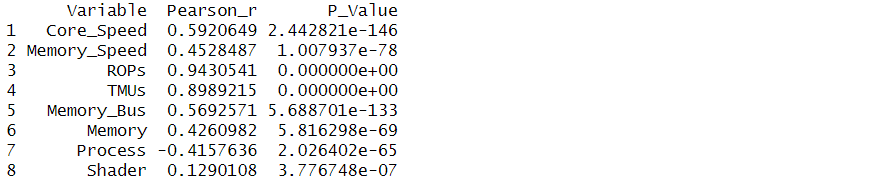
\includegraphics[width=1\linewidth]{images/Screenshot 2025-08-05 215207.png}}
\end{figure}

Như vậy, biến phụ thuộc Pixel\_Rate có quan hệ thống kê với tất cả các biến (p $<$ 0,001). Tuy nhiên với mục tiêu đơn giản hóa mô hình thì ta sẽ chọn những biến có  cao nhất là ROPs, Memory, TMUs, Core\_Speed và Memory\_Speed.

\subsection{Scatter plot và Scatter matrix}

\begin{figure}[!h]
    \centering
    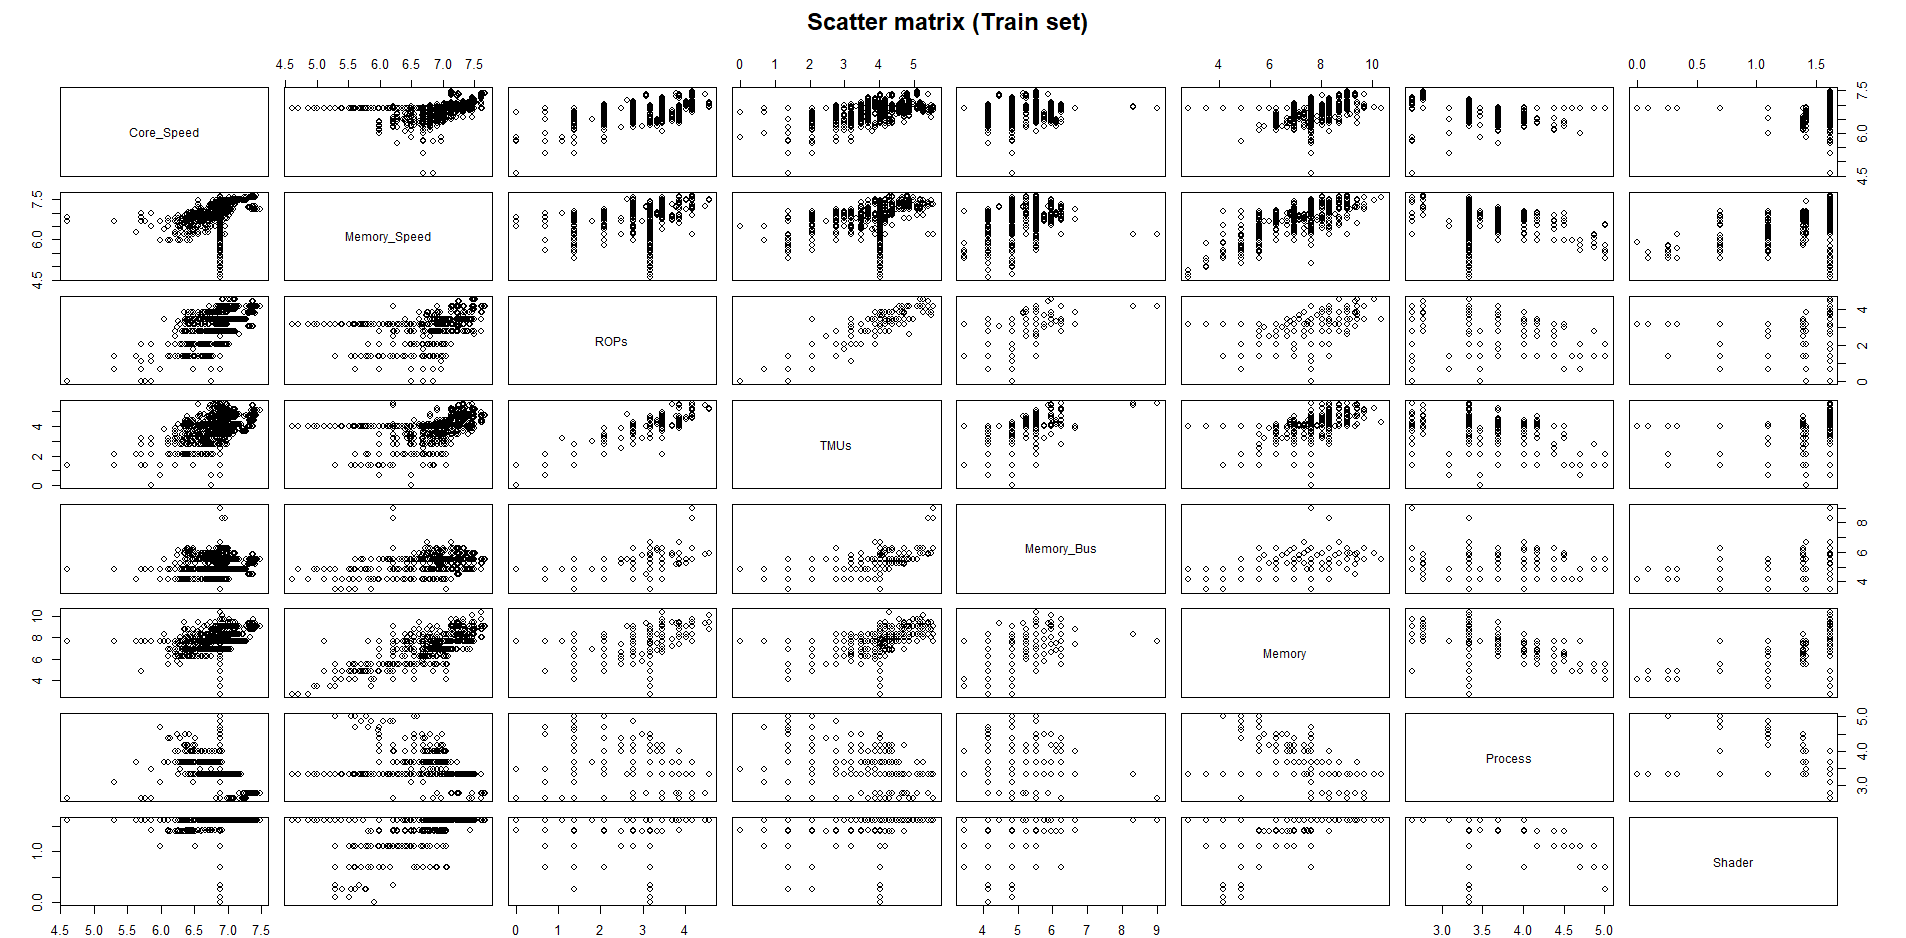
\includegraphics[width=1\linewidth]{images/Screenshot 2025-08-05 215544.png}
    \caption{Biểu đồ tương quan với hệ số tương quan giữa từng cặp biến}
\end{figure}

\section{Phân tích phương sai một yếu tố (ANOVA)}
Nhằm đánh giá sự khác biệt về hiệu suất xử lý đồ họa (Pixel\_Rate) giữa các nhóm phân loại khác nhau, Ta thực hiện phân tích phương sai (ANOVA một chiều) đối với ba biến phân loại chính Manufacturer, Memory\_Type và Resolution\_WxH trên tập huấn luyện (train).

\subsection{Mục tiêu}

\begin{itemize}
    \item Kiểm định xem liệu Pixel\_Rate có khác nhau giữa các nhóm phân loại (ví dụ Manufacturer) hay không, ở mức ý nghĩa $\alpha$ = 5%.
    \item Xác định xem có ít nhất một cặp nhóm có trung bình Pixel\_Rate khác biệt về mặt thống kê.
\end{itemize}

\subsection{Bài toán}

\subsubsection{Các điều kiện cần kiểm tra trước khi thực hiện ANOVA}

\textbf{Điều kiện 1:} Độc lập của các quan sát

Các giá trị Pixel\_Rate đo được từ mỗi nhóm (Manufacturer / Memory\_Type / Resolution\_WxH) phải được thu thập độc lập.
Kết luận: Do dữ liệu được ghi nhận từ các dòng GPU khác nhau, không có chồng lắp hay phụ thuộc, nên điều kiện này được thoả.

\textbf{Điều kiện 2:} Biến phụ thuộc là biến liên tục

Pixel\_Rate là giá trị số thực liên tục (Gpixel/s).
Kết luận: Điều kiện này được thoả.

\textbf{Điều kiện 3:} Phân phối chuẩn trong mỗi nhóm

Dùng kiểm định Shapiro–Wilk trên phần dư hoặc trực tiếp trên từng nhóm.
Nếu $p>0.05$, phần dư (hoặc dữ liệu nhóm) xấp xỉ phân phối chuẩn.

\textbf{Điều kiện 4:} Đồng nhất phương sai giữa các nhóm
Dùng Levene’s test.

Nếu $p>0.05$, không bác bỏ giả thiết phương sai bằng nhau.

\subsubsection{Giả thuyết của bài toán}
$H_0$: Trung bình Pixel\_Rate của tất cả các nhóm là bằng nhau.
$$H_0: \mu_1 = \mu_2 = \cdots = \mu_k$$

\textbf{Ví dụ với Manufacturer:}

$H_1$: Có ít nhất một cặp nhóm có trung bình Pixel\_Rate khác nhau.
$$H_A: \exists i \neq j \text{ sao cho } \mu_i \neq \mu_j
$$

Sau khi xác nhận (1) - (4), ta tiến hành ANOVA một yếu tố để kiểm định $H_0$ ở mức ý nghĩa $\alpha=0.05$. Nếu $p < 0.05$, bác bỏ $H_0$, kết luận rằng có sự khác biệt về hiệu suất Pixel\_Rate giữa các nhóm.
\subsection{Kiểm định giả thuyết}
Trước khi thực hiện phân tích phương sai (ANOVA), hai giả định quan trọng cần được kiểm tra là phân phối chuẩn trong mỗi nhóm (điều kiện 3) và đồng nhất phương sai giữa các nhóm (điều kiện 4). Các kiểm định được sử dụng bao gồm Shapiro-Wilk để đánh giá phân phối chuẩn của phần dư và Levene’s test để kiểm tra đồng nhất phương sai. Dưới đây là kết quả kiểm tra cho từng biến phân loại: Manufacturer, Memory\_Type, và Resolution\_WxH.

\subsubsection{Biến Manufacturer}
\begin{itemize}
    \item \textbf{Kiểm định Shapiro-Wilk (phân phối chuẩn của phần dư):}
    
    \textbf{\textit{Thống kê:}} W = 0.96812
    
    \textbf{\textit{Giá trị:}} $p<2.2 \times10^{-16} $
    
    \textbf{\textit{Kết luận:}} Vì p $<$ 0.05, bác bỏ giả thuyết  rằng phần dư tuân theo phân phối chuẩn. Phần dư không xấp xỉ phân phối chuẩn.
    \item \textbf{Kiểm định Levene (đồng nhất phương sai):}
    
    \textit{\textbf{Thống kê:}} F(3, 1467) = 8.799

   \textit{\textbf{Giá trị:}} $p = 8.781 \times10^{-6} $
    
   \textit{\textbf{Kết luận:}} Vì $p < 0.05$, bác bỏ giả thuyết  rằng phương sai giữa các nhóm là bằng nhau. Phương sai không đồng nhất.
\end{itemize}

\subsubsection{Biến Memory\_Type}
\begin{itemize}
    \item \textbf{Kiểm định Shapiro-Wilk (phân phối chuẩn của phần dư):}
    
    \textbf{\textit{Thống kê:}} W = 0.97858

    \textbf{\textit{Giá trị:}} $p=5.408\cdot{10}^{-14}$
    
    \textbf{\textit{Kết luận:}} Vì p $<$ 0.05, bác bỏ giả thuyết . Phần dư không tuân theo phân phối chuẩn.
    \item \textbf{Kiểm định Levene (đồng nhất phương sai):}
    
    \textbf{\textit{Thống kê:}} F(3, 1467) = 24.659
    
   \textbf{\textit{Giá trị:}} $p=1.445\cdot{10}^{-15}$
    
    \textbf{\textit{Kết luận:}} Vì p $<$ 0.05, bác bỏ giả thuyết . Phương sai giữa các nhóm không đồng nhất.
\end{itemize}

\subsubsection{Biến Resolution\_WxH}

    \begin{itemize}
        \item K\textbf{iểm định Shapiro-Wilk (phân phối chuẩn của phần dư):}
        
        \textbf{\textit{Thống kê:}} W = 0.96255
        
        \textbf{\textit{Giá trị:}} $p<2.2\cdot{10}^{-16}$
        
        \textbf{\textit{Kết luận:}} Vì p $<$ 0.05, bác bỏ giả thuyết$ H_0$. Phần dư không xấp xỉ phân phối chuẩn.
        \item \textbf{Kiểm định Levene (đồng nhất phương sai):}
        
        \textbf{\textit{Thống kê:}} F(2, 1468) = 20.193
        
        \textbf{\textit{Giá trị:}} $p=2.232\cdot{10}^{-9}$
        
        \textbf{\textit{Kết luận:}} Vì p $<$ 0.05, bác bỏ giả thuyết $H_0$. Phương sai giữa các nhóm không đồng nhất.
    \end{itemize}

\newpage
\textbf{Dựa trên phân tích, ta có kết luận:}

Kết quả từ các kiểm định Shapiro-Wilk và Levene cho thấy cả hai giả định về phân phối chuẩn và đồng nhất phương sai đều không được thỏa mãn đối với các biến Manufacturer, Memory\_Type, và Resolution\_WxH (giá trị p $<$ 0.05 trong tất cả các trường hợp). Tuy nhiên, ANOVA vẫn có thể được tiến hành nhờ tính bền vững của phương pháp này với kích thước mẫu lớn $(n \approx 1470)$, giúp giảm thiểu tác động của các vi phạm giả định.

\subsection{Tiến hành phân tích phương sai và kết quả}
Ta sử dụng hàm aov() trong R để thực hiện phân tích phương sai một yếu tố (ANOVA) cho biến Pixel\_Rate, phân loại theo các biến Manufacturer, Memory\_Type, và \ trên tập dữ liệu huấn luyện (train). Kết quả của mỗi phân tích được in ra bằng hàm summary().

Ta xây dựng mô hình:

\begin{minted}{r}
for (cat in categorical) {
  cat("\nANOVA for", cat, "on Train set\n")
  aov_mod <- aov(as.formula(paste("Pixel_Rate ~", cat)), data = train)
  print(summary(aov_mod))
}
\end{minted}

\textbf{Kết quả phân tích phương sai}

Dưới đây là kết quả ANOVA cho từng biến phân loại:

\subsubsection{Biến Manufacturer}
\begin{figure}[!h]
    \centering
    \fbox{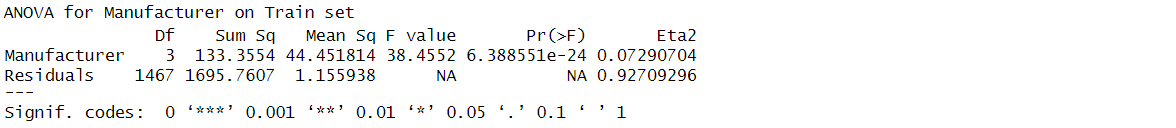
\includegraphics[width=1\linewidth]{images/Screenshot 2025-08-06 002901.png}}
\end{figure}

\textbf{Nhận xét:}

Giá trị F = 38.45 rất cao, cho thấy sự khác biệt lớn về trung bình Pixel\_Rate giữa các nhóm nhà sản xuất.

Giá trị $p < 2e-16$ (nhỏ hơn 0.05), bác bỏ giả thuyết $H_0$ rằng trung bình Pixel\_Rate của các nhà sản xuất là như nhau.

\subsubsection{Biến Memory\_Type}
\newpage
\begin{figure}[!h]
    \centering
    \fbox{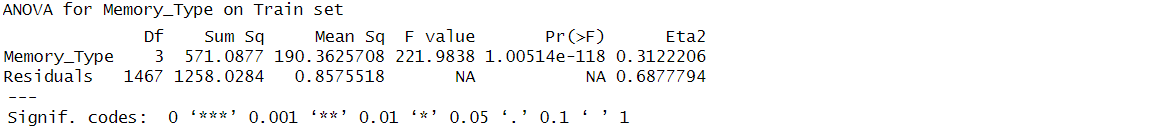
\includegraphics[width=1\linewidth]{images/Screenshot 2025-08-06 002942.png}}
\end{figure}

\textbf{Nhận xét:}

Giá trị F = 222 cực kỳ cao, cho thấy sự khác biệt đáng kể về trung bình Pixel\_Rate giữa các loại bộ nhớ.

Giá trị $p < 2e-16$, bác bỏ giả thuyết $H_0$ rằng trung bình Pixel\_Rate của các loại bộ nhớ là như nhau.

\subsubsection{Biến Resolution\_WxH}

\begin{figure}[!h]
    \centering
    \fbox{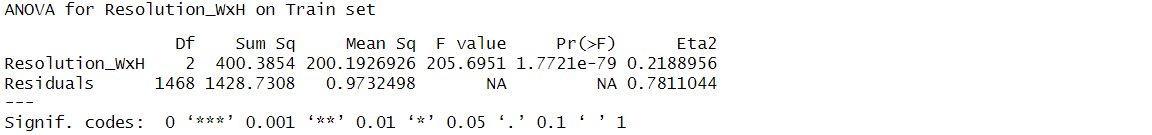
\includegraphics[width=1\linewidth]{images/Screenshot 2025-08-06 002957.png}}
\end{figure}

\textbf{Nhận xét:}

Giá trị F = 205.7 rất cao, cho thấy sự khác biệt lớn về trung bình Pixel\_Rate giữa các độ phân giải.

Giá trị$ p < 2e-16$, bác bỏ giả thuyết $H_0$ rằng trung bình Pixel\_Rate của các độ phân giải là như nhau.

\textbf{*Tổng hợp kết quả}

Dưới đây là bảng tổng hợp các giá trị đặc trưng của mô hình ANOVA cho từng biến:

\begin{longtable}{|l|c|c|c|c|}
\hline
\textbf{Biến} & \textbf{Df (giữa nhóm)} & \textbf{Df (trong nhóm)} & \textbf{Sum Sq (SSB)} & \textbf{Sum Sq (SSW)} \\
\hline
Manufacturer & 3 & 1467 & 133.4 & 1695.8 \\
\hline
Memory\_Type & 3 & 1467 & 571.1 & 1258.0 \\
\hline
Resolution\_WxH & 2 & 1468 & 400.4 & 1428.7 \\
\hline
\end{longtable}

\begin{longtable}{|l|c|c|c|c|}
\hline
\textbf{Biến}& \textbf{Mean Sq (MSB)} & \textbf{Mean Sq (MSW)} & \textbf{F value} & \textbf{p-value} \\
\hline
Manufacturer & 44.45 & 1.16 & 38.45 & $<$2e-16 \\
\hline
Memory\_Type & 190.36 & 0.86 & 222 & $<$2e-16 \\
\hline
Resolution\_WxH & 200.19 & 0.97 & 205.7 & $<$2e-16 \\
\hline
\end{longtable}

\newpage
\textbf{Ghi chú:}
\begin{itemize}
  \item \textbf{\textit{Df (giữa nhóm):}} Bậc tự do giữa các nhóm.
  \item \textbf{\textit{Df (trong nhóm):}} Bậc tự do trong nhóm (Residuals).
  \item \textbf{\textit{Sum Sq (SSB):}} Tổng bình phương giữa các nhóm.
  \item \textbf{\textit{Sum Sq (SSW):}} Tổng bình phương trong nhóm.
  \item \textbf{\textit{Mean Sq (MSB):}} Trung bình bình phương giữa các nhóm.
  \item \textbf{\textit{Mean Sq (MSW):}} Trung bình bình phương trong nhóm.
\end{itemize}

\subsection{Kết luận}

Cả ba biến đều có giá trị F rất cao: 38.45 (Manufacturer), 222 (Memory\_Type), 205.7 (Resolution\_WxH) và giá trị p $<$ 2e-16 cho cả ba biến, nhỏ hơn rất nhiều so với mức ý nghĩa thống kê $\alpha = 0.05$. Điều này cho thấy sự khác biệt rõ rệt về trung bình Pixel\_Rate giữa các nhóm theo từng biến, đồng thời ta bác bỏ giả thuyết $H_0$, kết luận rằng có sự khác biệt có ý nghĩa thống kê về Pixel\_Rate giữa các nhóm trong mỗi biến. Sự khác biệt này có thể xuất phát từ công nghệ sản xuất, chất lượng linh kiện, hoặc đặc điểm thiết kế của từng nhóm. Phân tích phương sai ANOVA cho thấy có sự khác biệt có ý nghĩa thống kê về Pixel\_Rate giữa các nhóm được chia theo biến Manufacturer, Memory\_Type, và Resolution\_WxH. Với giá trị F cao (38.45, 222, 205.7) và p-value $<$ 2e-16 cho cả ba biến. Và để làm rõ hơn về sự khác nhau này, ta sử dụng thêm câu lệnh TukeyHSD và vẽ đồ thị plot().

\subsection{Phân tích hậu nghiệm}

Để xác định cụ thể các cặp nhóm nào khác biệt đáng kể, ta tiến hành kiểm định hậu nghiệm Tukey HSD và tính toán effect size ($\eta^2$) nhằm đánh giá mức độ ảnh hưởng của từng biến đến sự biến động của Pixel\_Rate.

Ta sử dụng TukeyHSD(aov\_mod) để hậu nghiệm Tukey, tab[,"Sum Sq"] / sum(tab[ ,"Sum Sq"]) cho tính toán effect size và plot(TukeyHSD(aov\_mod), las = 1) để vẽ đồ thị:

\begin{minted}{r}
for (cat in categorical) {
  cat("\nANOVA for", cat, "on Train set\n")
  aov_mod <- aov(as.formula(paste("Pixel_Rate ~", cat)), data = train)  
  # 5.2.2 Hậu nghiệm Tukey & Effect size (η²)
  tukey_result <- TukeyHSD(aov_mod)
  print(tukey_result)
  plot(TukeyHSD(aov_mod), las = 1)
  tab <- summary(aov_mod)[[1]]
  eta2 <- tab[,"Sum Sq"] / sum(tab[,"Sum Sq"])
  print(cbind(tab, Eta2 = eta2))
}
\end{minted}

\subsubsection{Biến Manufacturer}

\textbf{Kết quả của Tukey HSD:}

\begin{figure}[!h]
    \centering
    \fbox{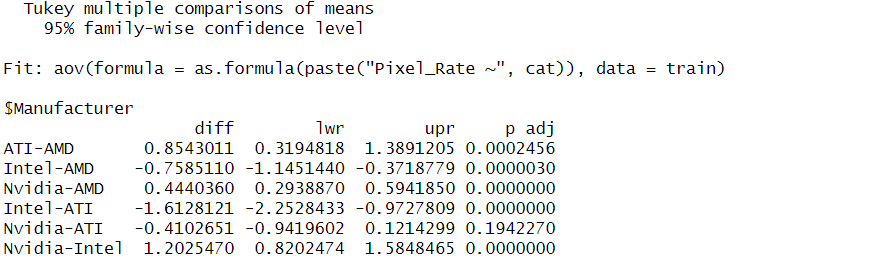
\includegraphics[width=1\linewidth]{images/Screenshot 2025-08-06 003238.png}}
\end{figure}

\textbf{Kết quả ANOVA và η²:}

\begin{figure}[!h]
    \centering
    \fbox{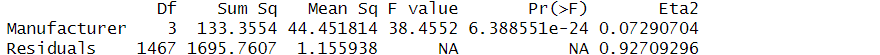
\includegraphics[width=1\linewidth]{images/Screenshot 2025-08-06 003246.png}}
\end{figure}

\textbf{Đồ thị Tukey HSD:}

\begin{figure}[!h]
    \centering
    \fbox{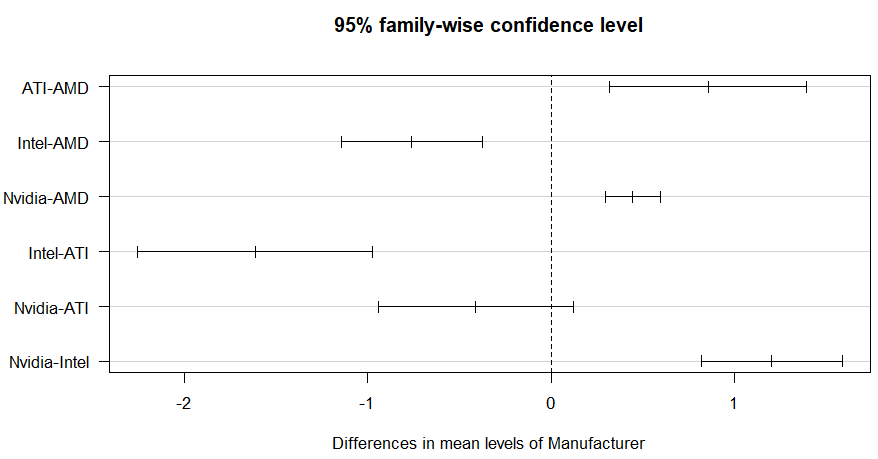
\includegraphics[width=1\linewidth]{images/Screenshot 2025-08-06 003404.png}}
\end{figure}

\newpage
\textbf{Nhận xét:}

Các cặp có $p adj < 0.05$ (có sự khác biệt đáng kể): ATI-AMD, Intel-AMD, Nvidia-AMD, Intel-ATI, và Nvidia-Intel. Riêng cặp Nvidia-ATI có p adj = 0.1942270 > 0.05, nên không có sự khác biệt đáng kể.
    \begin{itemize}
        \item \textbf{\textit{ATI-AMD:}} Giá trị diff = 0.8543011 $>$ 0, khoảng tin cậy (0.3194818, 1.3891205) không bao gồm 0, cho thấy Pixel\_Rate trung bình của ATI lớn hơn AMD $({\bar{x}}\_{ATI}$ $>$ ${\bar{x}}\_{AMD})$.
        \item \textbf{\textit{Intel-AMD:}} Giá trị diff = -0.7585110 $<$ 0, khoảng tin cậy (-1.1451440, -0.3718779) không bao gồm 0, cho thấy Pixel\_Rate trung bình của Intel nhỏ hơn AMD $({\bar{x}}\_{Intel} < {\bar{x}}\_{AMD})$.
        \item \textbf{\textit{Nvidia-AMD:}} Giá trị diff = 0.4440360 $>$ 0, khoảng tin cậy (0.2938870, 0.5941850) không bao gồm 0, cho thấy Pixel\_Rate trung bình của Nvidia lớn hơn AMD $({\bar{x}}\_{Nvidia}$ $>$ ${\bar{x}}\_{AMD})$.
        \item \textbf{\textit{Intel-ATI:}} Giá trị diff = -1.6128121 $<$ 0, khoảng tin cậy (-2.2528433, -0.9727809) không bao gồm 0, cho thấy Pixel\_Rate trung bình của Intel nhỏ hơn ATI $({\bar{x}}\_{Intel} < {\bar{x}}\_{ATI})$.
        \item \textbf{\textit{Nvidia-ATI:}} Giá trị diff = -0.4102651, khoảng tin cậy (-0.9419602, 0.1214299) bao gồm 0, phù hợp với p adj $>$ 0.05, không có sự khác biệt đáng kể.
        \item \textbf{\textit{Nvidia-Intel:}} Giá trị diff = 1.2025470 $>$ 0, khoảng tin cậy (0.8202474, 1.5848465) không bao gồm 0, cho thấy Pixel\_Rate trung bình của Nvidia lớn hơn Intel $({\bar{x}}\_{Nvidia}$ $>$ ${\bar{x}}\_{Intel})$.
    \end{itemize}
    
Từ các kết quả trên, thứ tự Pixel\_Rate trung bình là:

\begin{center}
\boxed{\textit{\textbf{ATI $>$ Nvidia $>$ AMD $>$ Intel}}}    
\end{center}
    
\textbf{Effect size (η²):} Giá trị η² = 0.0729, cho thấy biến Manufacturer giải thích khoảng 7.29\% sự biến thiên của Pixel\_Rate.

\textbf{Đồ thị Tukey HSD:} Đồ thị cho thấy các khoảng tin cậy của ATI-AMD, Intel-AMD, Nvidia-AMD, Intel-ATI, và Nvidia-Intel không giao với đường x = 0, xác nhận sự khác biệt có ý nghĩa thống kê. Riêng Nvidia-ATI có khoảng tin cậy cắt qua 0, phù hợp với kết quả không đáng kể.

\subsubsection{Biến Memory\_Type}

\textbf{Kết quả của Tukey HSD:}

\begin{figure}[!h]
    \centering
    \fbox{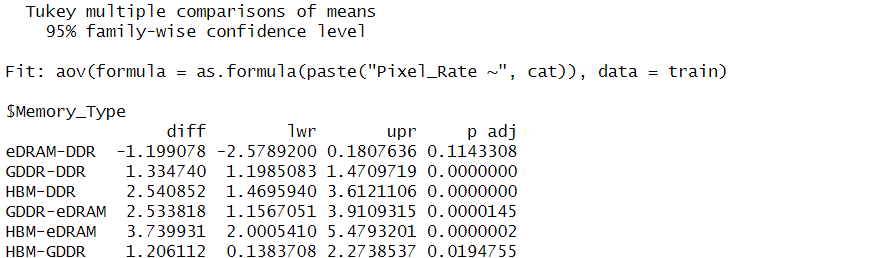
\includegraphics[width=1\linewidth]{images/Screenshot 2025-08-06 003257.png}}
\end{figure}

\textbf{Kết quả ANOVA và η²:}

\begin{figure}[!h]
    \centering
    \fbox{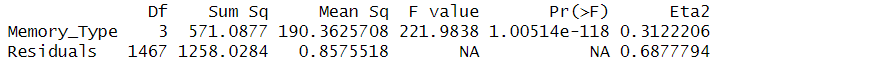
\includegraphics[width=1\linewidth]{images/Screenshot 2025-08-06 003304.png}}
\end{figure}

\textbf{Đồ thị Tukey HSD:}

\begin{figure}[!h]
    \centering
    \fbox{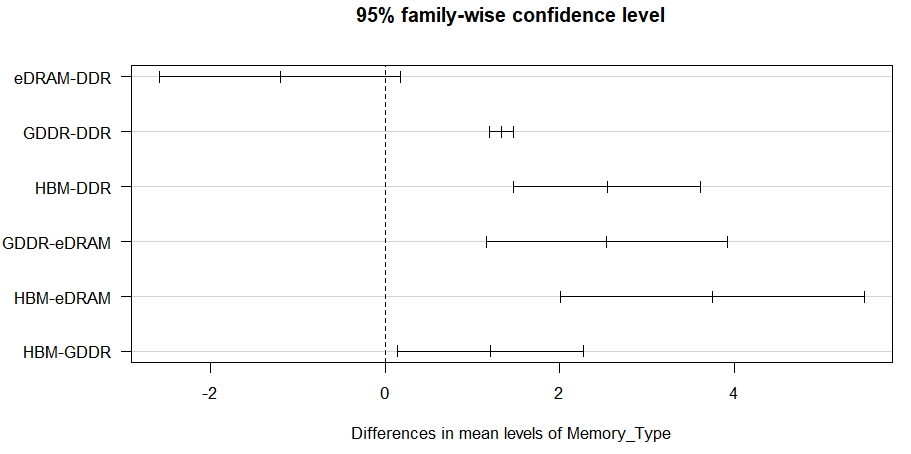
\includegraphics[width=1\linewidth]{images/Screenshot 2025-08-06 003419.png}}
\end{figure}

\textbf{Nhận xét:} Các cặp có $p adj < 0.05$ (có sự khác biệt đáng kể): \textit{GDDR-DDR, HBM-DDR, GDDR-eDRAM, HBM-eDRAM,} và \textit{HBM-GDDR}. Riêng cặp eDRAM-DDR có p adj = 0.1143308 > 0.05, không có sự khác biệt đáng kể.
    \begin{itemize}
        \item \textbf{\textit{GDDR-DDR:}} Giá trị diff$ = 1.334740 > 0$, khoảng tin cậy (1.1985083, 1.4709719) không bao gồm 0, cho thấy Pixel\_Rate trung bình của GDDR lớn hơn DDR $({\bar{x}}\_{GDDR}> {\bar{x}}\_{DDR})$.
        \item \textbf{\textit{HBM-DDR:}} Giá trị diff$ = 2.540852 > 0$, khoảng tin cậy (1.4695940, 3.6121106) không bao gồm 0, cho thấy Pixel\_Rate trung bình của HBM lớn hơn DDR $({\bar{x}}\_{HBM} > {\bar{x}}\_{DDR})$.
        \item \textbf{\textit{GDDR-eDRAM:}} Giá trịdiff  $= 2.533818 > 0$, khoảng tin cậy (1.1567051, 3.9109315) không bao gồm 0, cho thấy Pixel\_Rate trung bình của GDDR lớn hơn eDRAM $({\bar{x}}\_{GDDR} > {\bar{x}}\_{eDRAM})$.
        \item \textbf{\textit{HBM-eDRAM:}} Giá trị diff $= 3.739931 > 0$, khoảng tin cậy (2.0005410, 5.4793201) không bao gồm 0, cho thấy Pixel\_Rate trung bình của HBM lớn hơn eDRAM $({\bar{x}}\_{HBM} > {\bar{x}}\_{eDRAM})$.
        \item \textbf{\textit{HBM-GDDR:}} Giá trị diff$ = 1.206112 > 0$, khoảng tin cậy (0.1383708, 2.2738537) không bao gồm 0, cho thấy Pixel\_Rate trung bình của HBM lớn hơn GDDR $({\bar{x}}\_{HBM} > {\bar{x}}\_{GDDR})$.
    \end{itemize}
    
Từ các kết quả trên, thứ tự Pixel\_Rate trung bình là:

\begin{center}
    \boxed{\textbf{\textit{HBM $>$ GDDR $>$ DDR $>$ eDRAM}}}
\end{center}


\textbf{Effect size (η²):} Giá trị η² = 0.3122, cho thấy biến Memory\_Type giải thích khoảng 31.22\% sự biến thiên của Pixel\_Rate, mức ảnh hưởng khá lớn.

\textbf{Đồ thị Tukey HSD:} Đồ thị cho thấy các khoảng tin cậy của GDDR-DDR, HBM-DDR, GDDR-eDRAM, HBM-eDRAM, và HBM-GDDR không giao với đường x = 0, xác nhận sự khác biệt có ý nghĩa thống kê. Riêng eDRAM-DDR có khoảng tin cậy cắt qua 0, phù hợp với kết quả không đáng kể.

\subsubsection{Biến Resolution\_WxH}

\textbf{Kết quả của Tukey HSD:}

\begin{figure}[!h]
    \centering
    \fbox{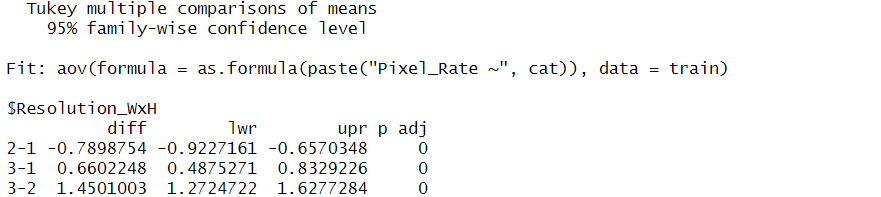
\includegraphics[width=1\linewidth]{images/Screenshot 2025-08-06 003315.png}}
\end{figure}

\newpage

\textbf{Kết quả ANOVA và η²:}

\begin{figure}[!h]
    \centering
    \fbox{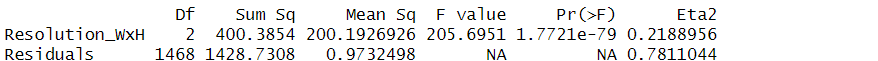
\includegraphics[width=1\linewidth]{images/Screenshot 2025-08-06 003323.png}}
\end{figure}

\textbf{Đồ thị Tukey HSD:}

\begin{figure}[!h]
    \centering
    \fbox{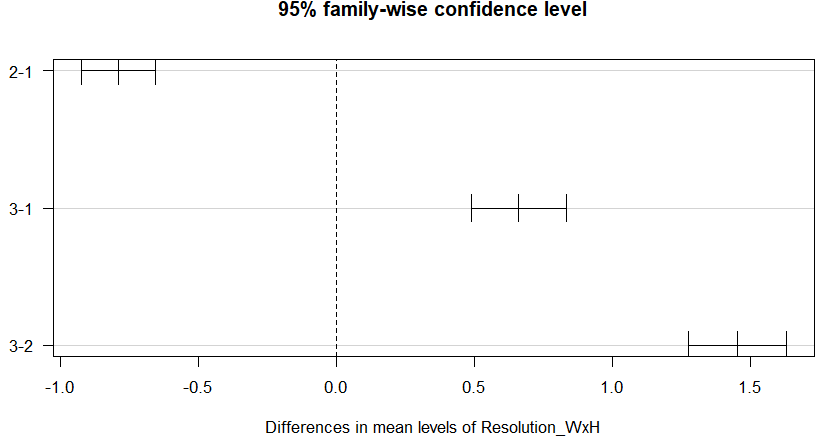
\includegraphics[width=1\linewidth]{images/Screenshot 2025-08-06 003429.png}}
\end{figure}

\textbf{Nhận xét:}

Tất cả các cặp đều có $p adj = 0 < 0.05$, cho thấy có sự khác biệt đáng kể giữa các nhóm.
    \begin{itemize}
        \item \textbf{\textit{2-1:}} Giá trị diff $= -0.7898754 < 0$, khoảng tin cậy (-0.9227161, -0.6570348) không bao gồm 0, cho thấy Pixel\_Rate trung bình của nhóm 2 nhỏ hơn nhóm 1 $({\bar{x}}\_2< {\bar{x}}\_1)$.
        \item \textbf{\textit{3-1:}} Giá trị diff $= 0.6602248 > 0$, khoảng tin cậy (0.4875271, 0.8329226) không bao gồm 0, cho thấy Pixel\_Rate trung bình của nhóm 3 lớn hơn nhóm 1 $({\bar{x}}\_3 > {\bar{x}}\_1)$.
        \item \textbf{\textit{3-2:}} Giá trị diff $= 1.4501003 > 0$, khoảng tin cậy (1.2724722, 1.6277284) không bao gồm 0, cho thấy Pixel\_Rate trung bình của nhóm 3 lớn hơn nhóm 2 $({\bar{x}}\_3 > {\bar{x}}\_2)$.
    \end{itemize}
    
Từ các kết quả trên, thứ tự Pixel\_Rate trung bình là:
\begin{center}
    \boxed{\textbf{\textit{Resolution 3 $>$ Resolution 1 $>$ Resolution 2}}}
\end{center}

\textbf{Effect size (η²):} Giá trị η² = 0.2189, cho thấy biến Resolution\_WxH giải thích khoảng 21.89\% sự biến thiên của Pixel\_Rate, mức ảnh hưởng đáng kể.

\textbf{Đồ thị Tukey HSD:} Đồ thị cho thấy tất cả các khoảng tin cậy của 2-1, 3-1, và 3-2 không giao với đường x = 0, xác nhận sự khác biệt có ý nghĩa thống kê giữa các nhóm.

\subsubsection{Kết luận}

Kết quả kiểm định hậu nghiệm Tukey HSD và effect size η² cho thấy:
\begin{itemize}
    \item \textbf{Manufacturer:} Có sự khác biệt đáng kể giữa các nhà sản xuất, với ATI có Pixel\_Rate trung bình cao nhất, nhưng η² = 0.0729 cho thấy biến này chỉ giải thích một phần nhỏ (7.29\%) sự biến thiên của Pixel\_Rate.
    \item \textbf{Memory\_Type:} Có sự khác biệt lớn giữa các loại bộ nhớ, với HBM có Pixel\_Rate trung bình cao nhất, và η² = 0.3122 cho thấy biến này có ảnh hưởng mạnh (31.22\%) đến Pixel\_Rate.
    \item \textbf{Resolution\_WxH:} Có sự khác biệt đáng kể giữa các nhóm độ phân giải, với nhóm 3 có Pixel\_Rate trung bình cao nhất, và η² = 0.2189 cho thấy biến này có ảnh hưởng đáng kể (21.89\%) đến Pixel\_Rate.
\end{itemize}
    
Kết quả này có thể được sử dụng để đánh giá tác động của các yếu tố phân loại lên hiệu suất GPU (Pixel\_Rate), từ đó hỗ trợ trong việc xây dựng mô hình hồi quy tuyến tính dự báo về sự phát triển của GPU trong mảng hiệu suất dựng ảnh.

\section{Xây dựng mô hình hồi quy đa biến}

Vấn đề đặt ra là tìm hiểu những yếu tố ảnh hưởng đến hiệu suất dựng ảnh Pixel\_Rate của GPU. Ta sẽ xây dựng mô hình hồi quy tuyến tính đa biến để giải quyết vấn đề này.
    
Mô hình hồi quy đa biến có dạng:
$$Y = \beta_0 + \beta_1 X_1 + \beta_2 X_2 + \cdots + \beta_n X_n + \epsilon$$

Đầu tiên, ta thực hiện chia tập dữ liệu thành tập train và test với tỉ lệ 2:1 và xây dựng mô hình hồi quy tuyến tính, lưu kết quả vào biến model:

\begin{minted}{r}
# Chia dữ liệu thành tập huấn luyện và tập kiểm tra (2/3 - 1/3)
set.seed(123)
index <- createDataPartition(GPU_new_log$Pixel_Rate, p = 2/3, list = FALSE)
train <- GPU_new_log[index, ]
test  <- GPU_new_log[-index, ]
\end{minted}

\subsection{Kiểm tra lại các biến}
Trước khi xây dựng mô hình hồi quy tuyến tính đa biến để dự đoán Pixel\_Rate, ta tiến hành các bước kiểm tra dữ liệu và lựa chọn biến nhằm đảm bảo mô hình đạt độ chính xác cao, tránh hiện tượng đa cộng tuyến và tối ưu hóa hiệu suất. Quá trình này bao gồm kiểm tra đa cộng tuyến bằng VIF, lựa chọn biến bằng phương pháp stepwise selection, và áp dụng feature engineering (đã làm ở trên bước xử lí dữ liệu và thống kê mô tả) để cải thiện chất lượng dữ liệu.

\subsubsection{Kiểm tra đa cộng tuyến bằng VIF}
Ta bắt đầu bằng cách xây dựng một mô hình hồi quy đầy đủ bao gồm tất cả các biến định lượng (Core\_Speed, Memory\_Speed, ROPs, TMUs, Memory\_Bus, Memory, Process, Shader) và biến phân loại (Manufacturer, Memory\_Type, Resolution\_WxH). Hệ số VIF (Variance Inflation Factor) được tính toán để kiểm tra hiện tượng đa cộng tuyến giữa các biến, sử dụng đoạn mã sau:

\begin{minted}{r}
# Tạo công thức với tất cả biến
full_form <- as.formula(
  paste("Pixel_Rate ~", paste(c(numerical, categorical), collapse = " + "))
)
# Huấn luyện mô hình đầy đủ
full_mod <- lm(full_form, data = train)
print(vif(full_mod))  # Kiểm tra multicollinearity
\end{minted}

Kết quả thu được sau khi ta chạy đoạn mã:
\begin{figure}[!h]
    \centering
    \fbox{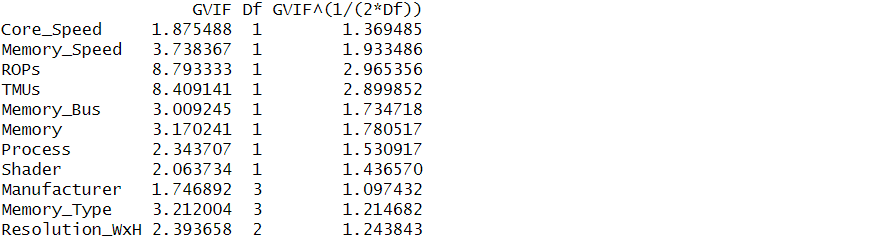
\includegraphics[width=1\linewidth]{images/Screenshot 2025-08-06 010408.png}}
\end{figure}

Các biến có VIF $<$ 5 thường được coi là không có đa cộng tuyến nghiêm trọng. Tuy nhiên, hai biến ROPs (VIF = 8.79) và TMUs (VIF = 8.41) có giá trị VIF cao, cho thấy tồn tại đa cộng tuyến giữa các biến này. Điều này có thể ảnh hưởng đến độ tin cậy của các hệ số hồi quy, do đó cần xem xét thêm trong quá trình lựa chọn biến.

\subsubsection{Lựa chọn biến bằng stepwise selection}

Để tối ưu hóa mô hình, ta sử dụng phương pháp stepwise selection (hướng "both") nhằm tự động lựa chọn các biến có ý nghĩa thống kê và loại bỏ các biến không cần thiết. Phương pháp này cải thiện độ chính xác và đơn giản hóa mô hình. Đoạn mã được sử dụng:

\begin{minted}{r}
# Lựa chọn biến bằng stepwise selection
step_mod <- step(full_mod, direction = "both", trace = 0)
print(summary(step_mod))
\end{minted}

Kết quả mô hình sau khi áp dụng stepwise selection:

\begin{figure}[!h]
    \centering
    \fbox{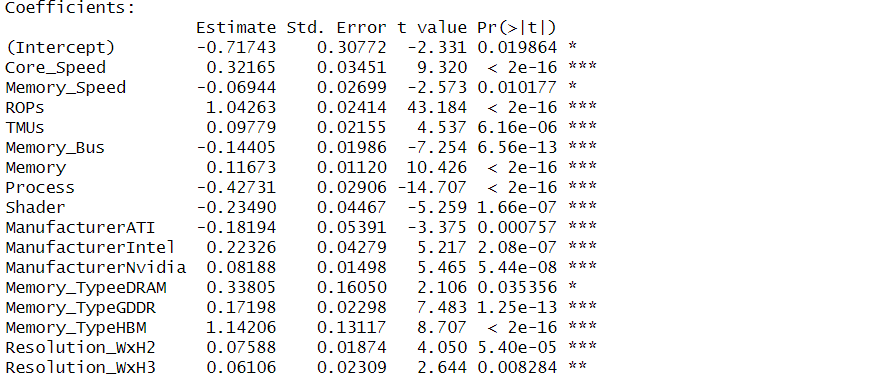
\includegraphics[width=1\linewidth]{images/Screenshot 2025-08-06 010632.png}}
\end{figure}

Sau khi áp dụng stepwise selection, mô hình vẫn giữ lại tất cả các biến ban đầu, điều này cho thấy các biến đều có ý nghĩa thống kê (p-value $<$ 0.05) trong việc dự đoán Pixel\_Rate. Tất cả các biến ban đầu đều được giữ lại, với các hệ số hồi quy có ý nghĩa thống kê cao, cho thấy chúng đóng vai trò quan trọng trong việc giải thích Pixel\_Rate.

\subsection{Xây dựng mô hình đa biến}

Ta xây dựng mô hình hồi quy tuyến tính đa biến để dự đoán Pixel\_Rate dựa trên các biến độc lập bao gồm các biến định lượng (Core\_Speed, Memory\_Speed, ROPs, TMUs, Memory\_Bus, Memory, Process, Shader) và các biến phân loại (Manufacturer, Memory\_Type, Resolution\_WxH). Mô hình được huấn luyện trên tập dữ liệu train, và kết quả được phân tích thông qua hàm summary(model\_final):

\begin{minted}{r}
# 5.3.2 Xây dựng mô hình đa biến
model_final <- step_mod
print(summary(model_final))
\end{minted}

\begin{figure}[!h]
    \centering
    \fbox{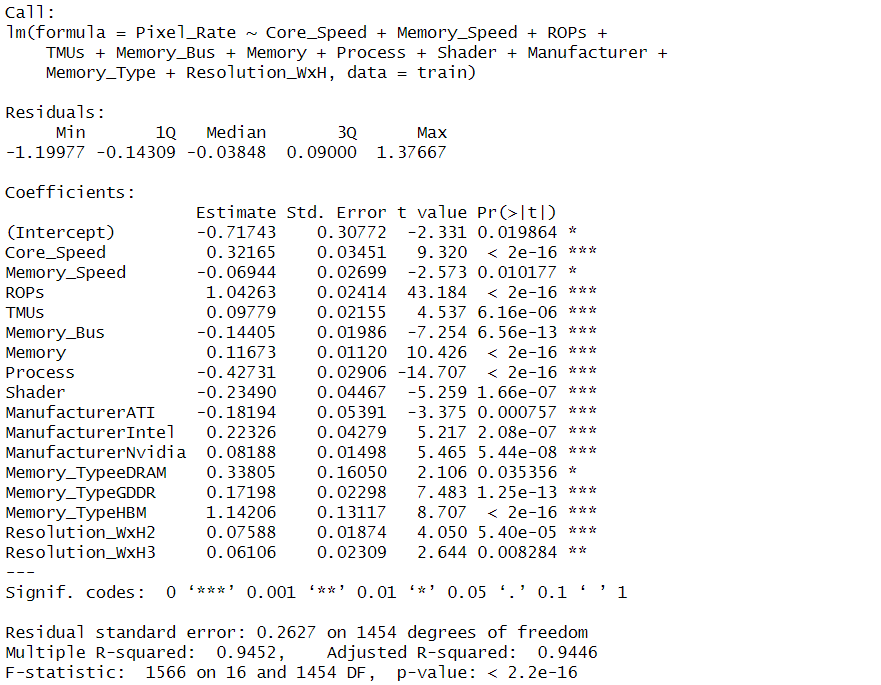
\includegraphics[width=0.75\linewidth]{images/Screenshot 2025-08-06 010852.png}}
\end{figure}

\textbf{Nhận xét:}

\begin{itemize}
    \item \textbf{Hệ số hồi quy:}
    \begin{itemize}
    \item \textbf{\textit{Intercept:}} Hệ số chặn của mô hình là -0.71743, cho biết giá trị kỳ vọng của Pixel\_Rate khi tất cả các biến dự báo bằng 0. Tuy nhiên, giá trị này có thể không mang ý nghĩa thực tiễn trong bối cảnh thực tế.
    \item \textbf{\textit{Core\_Speed:}} Hệ số hồi quy là 0.32165, cho biết khi Core\_Speed tăng thêm một đơn vị (giả sử các biến khác không thay đổi), Pixel\_Rate tăng trung bình 0.32165 đơn vị.
    \item \textbf{\textit{Memory\_Speed:}} Hệ số hồi quy là -0.06944, cho thấy khi Memory\_Speed tăng thêm một đơn vị, Pixel\_Rate giảm trung bình 0.06944 đơn vị.
    \item \textbf{\textit{ROPs:}} Hệ số hồi quy là 1.04263, cho thấy khi ROPs tăng thêm một đơn vị, Pixel\_Rate tăng trung bình 1.04263 đơn vị, thể hiện ảnh hưởng mạnh mẽ của biến này.
    \item \textbf{\textit{TMUs:}} Hệ số hồi quy là 0.09779, cho biết khi TMUs tăng thêm một đơn vị, Pixel\_Rate tăng trung bình 0.09779 đơn vị.
    \item \textbf{\textit{Memory\_Bus:}} Hệ số hồi quy là -0.14405, cho thấy khi Memory\_Bus tăng thêm một đơn vị, Pixel\_Rate giảm trung bình 0.14405 đơn vị.
    \item \textbf{\textit{Memory:}} Hệ số hồi quy là 0.11673, nghĩa là khi Memory tăng thêm một đơn vị, Pixel\_Rate tăng trung bình 0.11673 đơn vị.
    \item \textbf{\textit{Process:}} Hệ số hồi quy là -0.42731, cho biết khi Process tăng thêm một đơn vị, Pixel\_Rate giảm trung bình 0.42731 đơn vị.
    \item \textbf{\textit{Shader:}} Hệ số hồi quy là -0.23490, cho thấy khi Shader tăng thêm một đơn vị, Pixel\_Rate giảm trung bình 0.23490 đơn vị.
    \item \textbf{\textit{Manufacturer:}}
    \begin{itemize}
    \item \textbf{\textit{ManufacturerATI:}} Hệ số -0.18194, cho thấy Pixel\_Rate của ATI thấp hơn nhóm cơ sở.
    \item \textbf{\textit{ManufacturerIntel:}} Hệ số 0.22326, cho thấy Pixel\_Rate của Intel cao hơn nhóm cơ sở.
    \item \textbf{\textit{ManufacturerNvidia:}} Hệ số 0.08188, cho thấy Pixel\_Rate của Nvidia cao hơn nhóm cơ sở.
\end{itemize}
    \item \textbf{\textit{Memory\_Type:}}
\begin{itemize}
    \item \textbf{\textit{Memory\_TypeeDRAM:}} Hệ số 0.33805, cho thấy Pixel\_Rate của eDRAM cao hơn nhóm cơ sở.
    \item \textbf{\textit{Memory\_TypeGDDR:}} Hệ số 0.17198, cho thấy Pixel\_Rate của GDDR cao hơn nhóm cơ sở.
    \item \textbf{\textit{Memory\_TypeHBM:}} Hệ số 1.14206, cho thấy Pixel\_Rate của HBM cao hơn đáng kể so với nhóm cơ sở.
\end{itemize}
\item \textbf{\textit{Resolution\_WxH:}}
\begin{itemize}
    \item \textbf{\textit{Resolution\_WxH2:}} Hệ số 0.07588, cho thấy Pixel\_Rate của nhóm 2 cao hơn nhóm cơ sở.
    \item \textbf{\textit{Resolution\_WxH3:}} Hệ số 0.06106, cho thấy Pixel\_Rate của nhóm 3 cao hơn nhóm cơ sở.
\end{itemize}
\end{itemize}
\item \textbf{Ý nghĩa thống kê:}

Các giá trị p-value của tất cả các biến độc lập đều nhỏ hơn 0.05, cho thấy các biến này có ảnh hưởng ý nghĩa thống kê đến Pixel\_Rate ở mức ý nghĩa 5\%. Đặc biệt, các biến như ROPs, Process, Memory, và Core\_Speed có p-value $<$ 2e-16, thể hiện mức độ ý nghĩa thống kê rất cao.
\item \textbf{Độ phù hợp của mô hình:}
\begin{itemize}
    \item \textbf{\textit{Multiple R-squared:}} Giá trị ( $R^2$ = 0.9452 ), chỉ ra rằng khoảng 94.52\% phương sai của Pixel\_Rate được giải thích bởi mô hình hồi quy này. Đây là mức độ giải thích rất cao, cho thấy mô hình phù hợp tốt với dữ liệu.
    \item \textbf{\textit{Adjusted R-squared:}} Giá trị ( $R^2$ ) điều chỉnh là 0.9446, gần với ( $R^2$ ), cho thấy mô hình không bị overfitting dù có nhiều biến độc lập.
    \item \textbf{\textit{F-statistic:}} Giá trị F = 1566 với p-value $<$ 2.2e-16, xác nhận mô hình có ý nghĩa thống kê tổng thể.
\end{itemize}

\item \textbf{Phần dư (Residuals)}

Phần dư dao động từ -1.19977 đến 1.37667, với độ lệch chuẩn là 0.2627. Giá trị phần dư tương đối nhỏ, cho thấy mô hình dự đoán khá chính xác. Tuy nhiên, phần dư tối đa (1.37667) có thể chỉ ra rằng một số điểm dữ liệu chưa được giải thích hoàn toàn, có thể do thiếu các biến quan trọng khác.
\end{itemize}

\subsection{Đồ thị chuẩn đoán (Diagnostic plots)}

Sử dụng câu lệnh plot(model\_final) ta được 4 đồ thị như sau:

\begin{figure}[!h]
    \centering\fbox{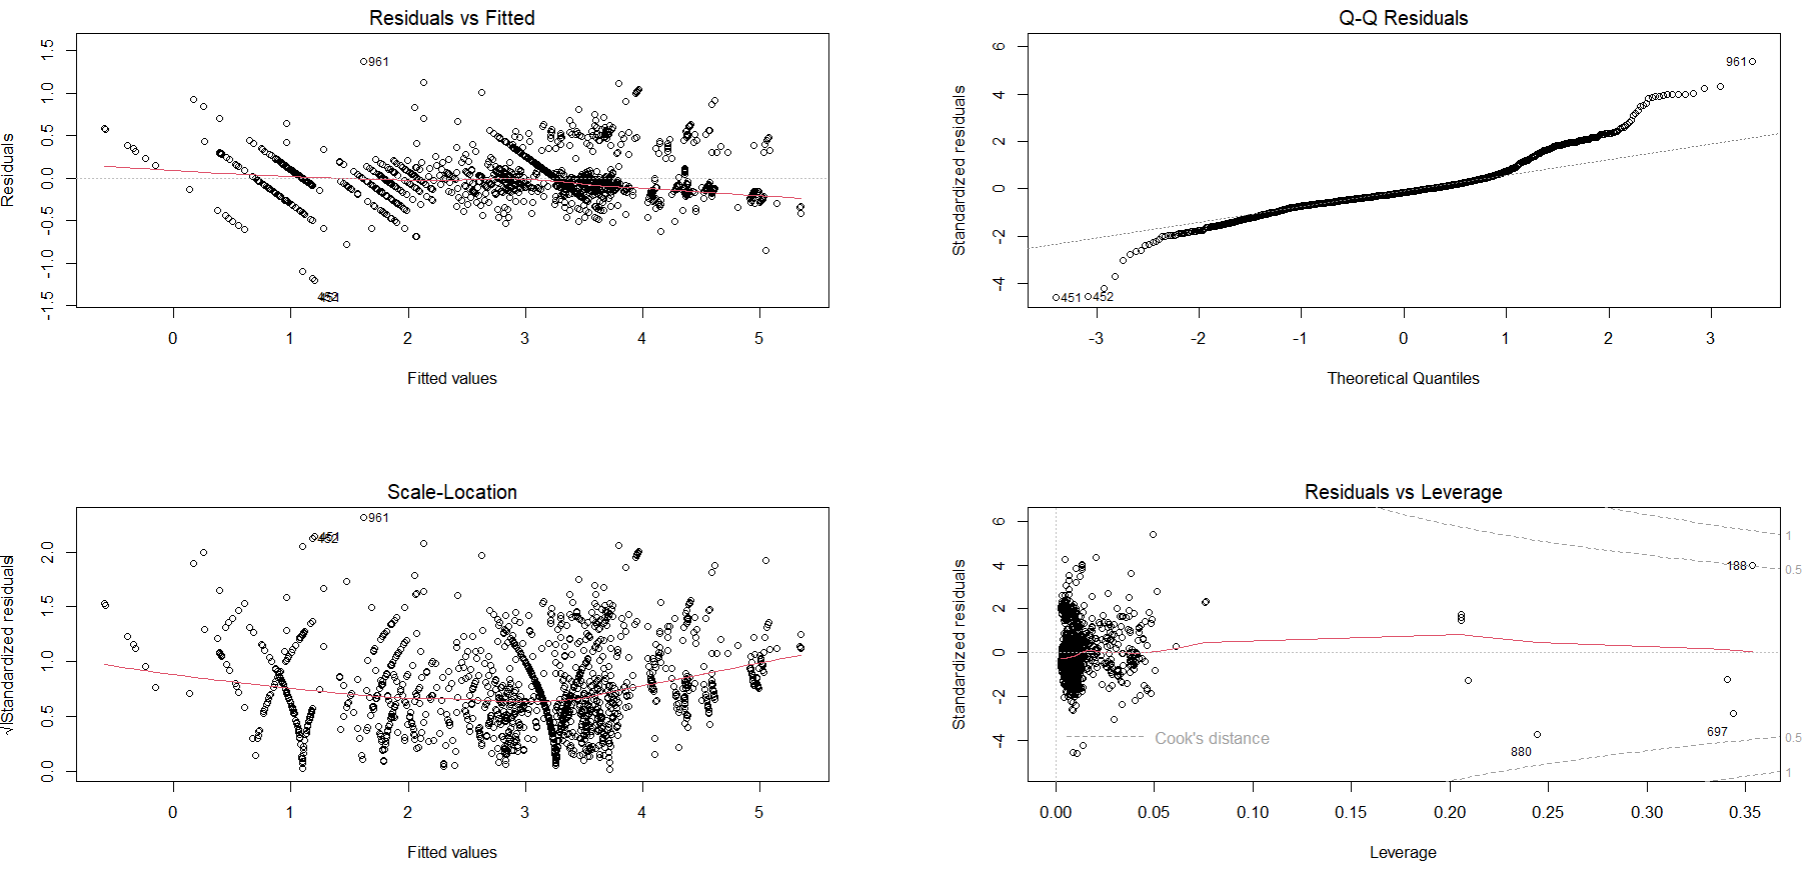
\includegraphics[width=1\linewidth]{images/Screenshot 2025-08-06 012450.png}}
\end{figure}
\newpage

\textbf{* Ta có nhận xét sau đây:}
\begin{itemize}
    \item \textbf{Đồ Thị 1 - Residuals vs Fitted:}
    
    Đồ thị này kiểm tra tính đồng nhất phương sai của phần dư (residuals) so với giá trị dự đoán (fitted values). Nếu phần dư phân bố ngẫu nhiên quanh đường zero, giả định đồng nhất phương sai có khả năng được thỏa mãn. Tuy nhiên, trong đồ thị này, ta quan sát thấy một mẫu hình rõ rệt: độ phân tán của phần dư tăng dần khi giá trị dự đoán tăng, đặc biệt sau mức giá trị 3. Một số điểm được đánh dấu như 961 và 1890 có phần dư lớn, cho thấy chúng có thể là các điểm ngoại lệ (outliers). Hiện tượng này gợi ý rằng mô hình đang gặp vấn đề về phương sai không đồng nhất (heteroscedasticity), tức là phương sai của phần dư không ổn định trên toàn bộ miền giá trị dự đoán.
    
    \item \textbf{Đồ Thị 2 - Normal Q-Q:}
    
    Đồ thị Normal Q-Q đánh giá xem phần dư có tuân theo phân phối chuẩn hay không. Nếu các điểm nằm gần đường thẳng lý thuyết, giả định phân phối chuẩn của phần dư được thỏa mãn. Ở đây, phần lớn các điểm nằm gần đường thẳng trong khoảng giữa (từ -2 đến 2), nhưng có sự lệch đáng kể ở hai đầu đuôi, đặc biệt tại các điểm như 491, 492 (đầu dưới) và 961 (đầu trên). Sự lệch này cho thấy phần dư có đuôi nặng hơn phân phối chuẩn, ám chỉ rằng giả định về tính chuẩn của phần dư không hoàn toàn được đáp ứng, đặc biệt với các giá trị cực đại hoặc cực tiểu.
    \item \textbf{Đồ Thị 3 - Scale-Location:}
    
    Đồ thị Scale-Location tiếp tục kiểm tra tính đồng nhất phương sai bằng cách biểu diễn căn bậc hai của phần dư chuẩn hóa so với giá trị dự đoán. Nếu phương sai đồng nhất, các điểm sẽ phân bố ngẫu nhiên quanh một đường ngang. Tuy nhiên, đồ thị này cho thấy một xu hướng tăng rõ ràng: độ phân tán của phần dư tăng khi giá trị dự đoán tăng, đặc biệt từ mức 3 trở lên. Các điểm như 961 và 1890 nổi bật với phần dư chuẩn hóa lớn. Xu hướng này củng cố bằng chứng về phương sai không đồng nhất (heteroscedasticity), xác nhận vấn đề đã phát hiện trong đồ thị Residuals vs Fitted.
    \item \textbf{Đồ Thị 4 - Residuals vs Leverage:}
    
    Đồ thị này giúp xác định các điểm ảnh hưởng mạnh (influential points) hoặc ngoại lệ bằng cách so sánh phần dư chuẩn hóa với giá trị đòn bẩy (leverage). Đa số các điểm có giá trị đòn bẩy thấp (gần 0), nhưng một số điểm như 880 và 857 có đòn bẩy cao (khoảng 0.3), và điểm 961 có cả phần dư lớn lẫn nằm gần hoặc vượt qua đường Cook’s distance 0.5. Những điểm này là các điểm ảnh hưởng mạnh tiềm năng, có thể tác động không nhỏ đến sự phù hợp của mô hình. Sự hiện diện của các điểm vượt qua ngưỡng Cook’s distance cho thấy cần xem xét kỹ hơn về ảnh hưởng của chúng.
\end{itemize}

\subsection{Đánh giá hiệu suất và sự ổn định của mô hình (sử dụng Cross-validation k‑fold)}

Để đánh giá khả năng tổng quát hóa và độ ổn định của mô hình hồi quy tuyến tính đa biến dự đoán Pixel\_Rate, ta thực hiện phương pháp cross-validation (k-fold) với k = 5. Quá trình này được thực hiện bằng cách sử dụng thư viện caret trong R, với đoạn mã như sau:

\begin{minted}{r}
# 5.3.4 Cross-validation (k-fold)
set.seed(123)
cv <- train(full_form, data = train,
            method = "lm",
            trControl = trainControl(method = "cv", number = 5))
print(cv)
\end{minted}

\begin{figure}[!h]
    \centering
    \fbox{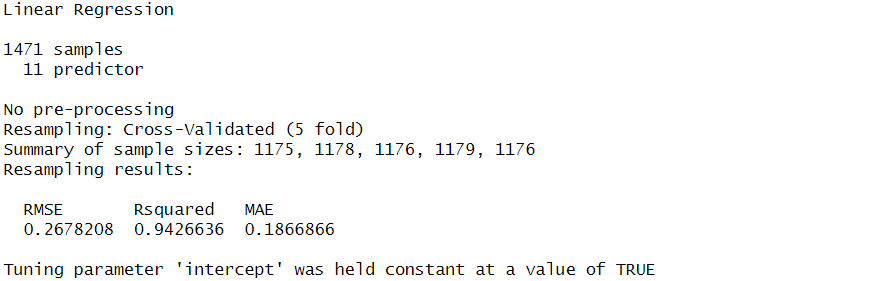
\includegraphics[width=1\linewidth]{images/Screenshot 2025-08-06 012927.png}}
\end{figure}

\textbf{Kết quả mà ta thu được từ quá trình cross-validation được trình bày như sau:}

\begin{itemize}
    \item \textbf{\textit{Số lượng mẫu:}} 1471 mẫu được sử dụng với 11 biến dự báo (predictors).
    \item \textbf{\textit{Phương pháp resampling:}} Cross-validated (5 fold), với kích thước mẫu trung bình của từng fold là khoảng 1175-1179 (tổng cộng 5 lần lặp).
    \item \textbf{Chỉ số đánh giá thu được:}
    \begin{itemize}
    \item \textbf{\textit{Giá trị RMSE}} trung bình là 0.2678208, phản ánh độ lệch trung bình của dự đoán so với giá trị thực tế. Đây là một chỉ số thấp, cho thấy mô hình có độ chính xác tốt trên các tập kiểm tra khác nhau.
    \item \textbf{\textit{Giá trị $\mathbf{R^2}$}} trung bình là 0.9426636, cho thấy mô hình giải thích được khoảng 94.27\% sự biến thiên của Pixel\_Rate trên các fold, thể hiện độ phù hợp cao và khả năng tổng quát hóa tốt.
    \item \textbf{\textit{Giá trị MAE}} trung bình là 0.1866866, chỉ ra sai số tuyệt đối trung bình giữa giá trị dự đoán và thực tế, củng cố thêm độ chính xác của mô hình.
\end{itemize}
    \item \textbf{Tham số điều chỉnh:} Tham số intercept được giữ cố định ở giá trị TRUE, không có pre-processing được áp dụng.
\end{itemize}

Nhận xét chung về kết quả thu được, ta thấy rằng mô hình hồi quy tuyến tính đa biến trên có hiệu suất ổn định và khả năng tổng quát hóa cao, với RMSE thấp (0.2678208) và $R^2$ cao (0.9426636) trên các fold khác nhau, điều này chứng tỏ rằng mô hình không bị quá khớp (overfitting) với tập huấn luyện. Giá trị MAE bằng 0.1866866 cũng bổ sung thêm bằng chứng về độ chính xác của mô hình, cho thấy sai số dự đoán là khá nhỏ. Ngoài ra, sự đồng nhất của các chỉ số trên 5 fold (dựa trên kích thước mẫu trung bình 1175-1179) cho thấy mô hình hoạt động ổn định trên các tập con khác nhau. Với kết quả thu được như trên, ta đánh giá được mô hình hồi quy tuyến tính đa biến trên là đáng tin cậy trong việc dự đoán Pixel\_Rate.

